\documentclass[english]{tumbeamer}

\usepackage{minted}
\usemintedstyle{colorful}
\usepackage{fontspec}

\setmonofont{JetBrainsMono}[
    Path=./jbmono/,
    Scale=0.85,
    Extension = .ttf,
    UprightFont=*-Regular,
    BoldFont=*-Bold,
    ItalicFont=*-Italic,
    BoldItalicFont=*-BoldItalic
    ]

\title{Docker, OCI containers}
\subtitle{VT Student Presentation }
\author{Roberto Castellotti}

\institute{\theDepartmentName\\\theUniversityName}
\date[06/12/2022]{December 6\textsuperscript{th}, 2022}
\footline{\insertauthor~|~\insertshorttitle~|~\insertshortdate}
\TUMbeamersetup{
  title page = TUM tower, 
  part page = TUM toc, 
  section page = TUM toc, 
  content page = TUM more space, 
  tower scale = 1.0,            
  headline = TUM threeliner,    
  footline = TUM default,       
  % configure on which pages headlines and footlines should be printed
  headline on = {title page},
  footline on = {every page, title page=false},
}

\begin{document}
\maketitle

\begin{frame}{History}
\begin{itemize}
    \item chroot
    \item freeBSD jails
    \item lxc/lxd
\end{itemize}
\end{frame}

\begin{frame}{chroot}
\begin{itemize}
    \item "Jails build upon the \texttt{chroot(2)} concept, which is used to change the root directory of a set of processes. This creates a safe environment, separate from the rest of the system. \textbf{Processes created in the chrooted environment cannot access files or resources outside of it}. For that reason, compromising a service running in a chrooted environment should not allow the attacker to compromise the entire system. However, a chroot has several limitations. It is suited to easy tasks which do not require much flexibility or complex, advanced features.
    \item Over time, \textbf{many ways have been found to escape from a chrooted environment}, making it a less than ideal solution for securing services."\footnote{https://docs.freebsd.org/en/books/handbook/jails/} 
\end{itemize}
\end{frame}

\begin{frame}{FreeBSD Jails (2000)}
Jails improve on the concept of the traditional chroot environment in several ways.
\begin{itemize}
    \item system resources
    \item system users
    \item running processes
    \item network stack
\end{itemize}
\vspace{5mm}
A jail has: 
\begin{itemize}
    \item a directory subtree
    \item a hostname
    \item an IP address
    \item a command to run
\end{itemize}
Root user is limited to the jail, this root account can't do anything on the host system.
\end{frame}

\begin{frame}{LXC}
Linux Containers (LXC) is an operating-system-level virtualization method for running multiple isolated Linux systems (containers) on a control host using a single Linux kernel.\footnote{https://en.wikipedia.org/wiki/LXC}.
Can be used for both System Containers and Application Containers
\vspace{3mm}
\begin{itemize}
    \item Kernel namespaces (ipc, uts, mount, pid, network and user)
    \item Apparmor and SELinux profiles
    \item Seccomp policies
    \item Chroots (using pivot\_root)
    \item Kernel capabilities
    \item CGroups (control groups)
\end{itemize}
\end{frame}

\begin{frame}{LXC/LXD (lxc:2008)}
LXD is a next generation system container and virtual machine manager. It offers a unified user experience around full Linux systems running inside containers or virtual machines.\footnote{https://linuxcontainers.org/lxd/introduction/}, Uses LXC for containers and Qemu for full virtualization.
\begin{figure}
    \centering
    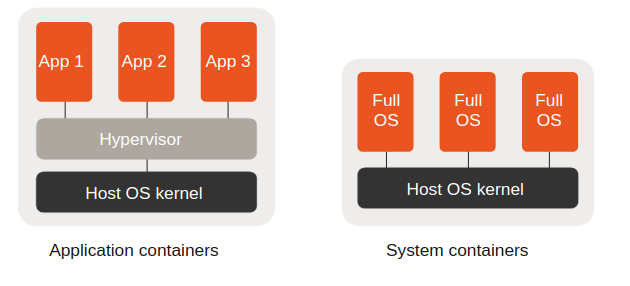
\includegraphics[width=0.6\textwidth]{application_vs_system.png}
    \caption{Application Containers (docker) vs System Containers (lxc)}
\end{figure}
\end{frame}

\begin{frame}{LXD}
A daemon, essentially the interface \texttt{lxc-*} commands interact with
\begin{itemize}
    \item Both supports VMS and System Containers.
    \item Should use System Containers (shared Kernel) when possible
    \item Should use Virtual VMs if:
        \begin{itemize}
            \item using a kernel feature not provided by host kernel
            \item using a different OS (of course)
        \end{itemize}
\end{itemize}
Probably the reason Docker had more success is this entire idea of "System Containers" is not really something needed in real world.
\end{frame}

\begin{frame}{"Docker"}
The \href{https://opencontainers.org/}{Open Container Initiative} is an open governance structure for the express purpose of creating open industry standards around container formats and runtimes.
\centering \begin{tabular}{ccc}

\includegraphics[width=.1\linewidth]{docker.png} & 

\includegraphics[width=.2\linewidth]{podman.png} & 

\includegraphics[width=.2\linewidth]{buildah.png}\\

\includegraphics[width=.2\linewidth]{skopeo.png} &

\includegraphics[width=.2\linewidth]{packer.png} &

\includegraphics[width=.2\linewidth]{kaniko.png}\\

\includegraphics[width=.2\linewidth]{containerd.png} & 

\includegraphics[width=.1\linewidth]{finch.png} & 
\end{tabular}
\end{frame}

\begin{frame}{Containers vs VMs (once again)}
\begin{figure}
    \centering
    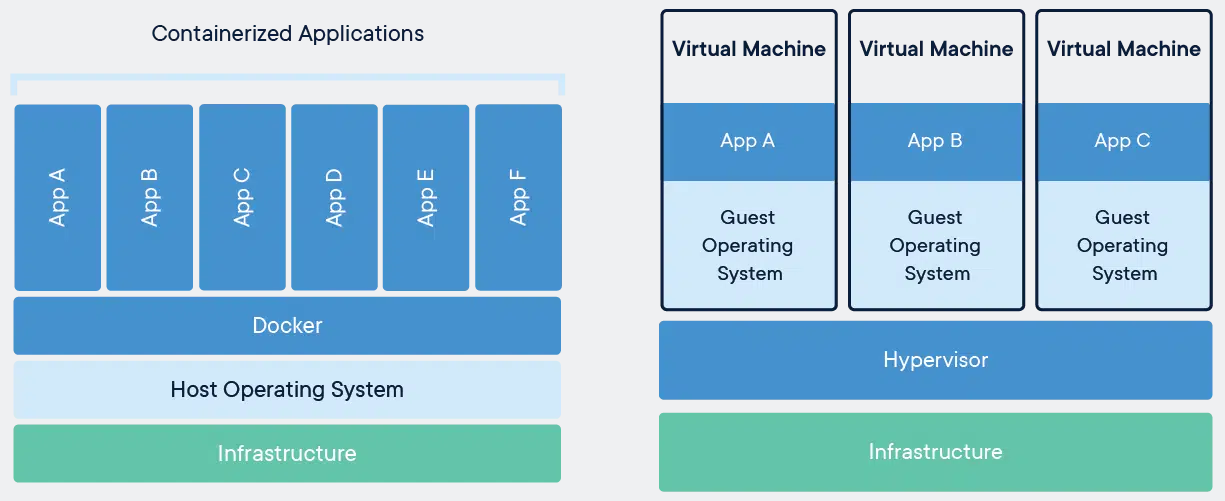
\includegraphics[width=0.8\textwidth]{container-vs-vms.png}
    \caption{from: https://www.docker.com/resources/what-container/ }
    \label{fig:my_label}
\end{figure}
\end{frame}

\begin{frame}{Open Container Initiative (OCI)}
The OCI was launched on June 22nd 2015 by Docker, CoreOS (Container Linux) and other leaders in the container industry. Currently 3 specifications:
\vspace{3mm}
\begin{itemize}
    \item the Runtime Specification (runtime-spec)
    \item the Image Specification (image-spec)
    \item the Distribution Specification (distribution-spec).
\end{itemize}
\vspace{3mm}
Docker donated its container format and runtime, runC (tool to spawn and run containers on linux), to the OCI to serve as the cornerstone of this new effort. It is available now at \href{https://github.com/opencontainers/runc}{opencontainers/runc}.
\end{frame}

\begin{frame}{How do containers provide isolation?}
"Applications are safer in containers and Docker provides the strongest default isolation capabilities in the industry" \footnote{\href{https://www.docker.com/resources/what-container/}{https://www.docker.com/resources/what-container/}}
\vspace{15mm}
\begin{itemize}
    \item linux namespaces (limits what you see)
    \item cgroups (limits what you can use use)
\end{itemize}
\end{frame}

\begin{frame}[fragile]{docker: quickstart}
\begin{itemize}
    \item create a Dockerfile:
    \begin{minted}{Dockerfile}
    FROM ubuntu:18.04
    COPY . /app
    RUN make /app
    CMD python /app/app.py
    \end{minted}
    \item \texttt{sudo docker build -t test . }
    \item \texttt{sudo docker run test } (ports? volumes?)
\end{itemize}
\vspace{3mm}
"Dockerfile" is supported also by other tools (podman, buildah) for compatibility reasons, while other tools, like HashiCorp Packer decided not to support them in order to not be tied to Docker in any way\footnote{https://developer.hashicorp.com/packer/plugins/builders/docker}
\end{frame}

\begin{frame}{How do we run containers in production?}
\begin{itemize}
    \item NOT \texttt{docker-compose}
    \item Docker Swarm, Kubernetes, Nomad orchestration tools
    \item "Kubernetes, also known as K8s, is an open-source system for automating deployment, scaling, and management of containerized applications." \footnote{https://kubernetes.io/}
    \item Usually managing a K8s cluster is not reccomended (huge complexity)
    \item Amazon EKS clusters, Azure AKS, Google GKE
    \item A lot of k8s distros: k8s is "only" a set (of huge) API specifications (minikube for local development, GKE for production)
    \item K8s and Nomad are big and powerful tools, use them only if needed! (HashiCorp Nomad scheduled 2,000,000 Docker containers on 6,100 hosts in 10 AWS regions in 22 minutes.)
    \item logging? backups? replicas? monitoring?
\end{itemize}
\end{frame}

\begin{frame}{Docker is lighter than a VM, or is it?}
\begin{itemize}
    \item microVMs:  provide enhanced security and workload isolation over traditional VMs, while enabling the speed and resource efficiency of containers. \footnote{https://firecracker-microvm.github.io/}
    \item \textbf{Firecracker}: KVM but no Qemu, custom VMM
    \item \textbf{Firecracker}: offers memory overhead of less than 5MB per container, boots to application code in less than 125ms, and
    allows creation of up to 150 MicroVMs per second per host.
    \item Why do we need this?
    \item \textbf{LightVM}: able to boot a (unikernel) VM in as little as 2.3ms, reach same-host VM densities of up to 8000 VMs
    \item \textbf{Unikernels}: tiny virtual machines where a minimalistic operating system (Unikraft)
    \item In some cases, a VM is lighter (and safer) than a container 
\end{itemize}
\end{frame}

\begin{frame}{further readings/talks}
\begin{itemize}
    \item \href{https://github.com/containerd/containerd/blob/main/docs/getting-started.md}{https://github.com/containerd/containerd/blob/main/docs/getting-started.md}
    \item \href{https://lwn.net/Articles/531114/}{https://lwn.net/Articles/531114/} (the entire series)
    \item \href{https://blog.quarkslab.com/digging-into-linux-namespaces-part-1.html}{https://blog.quarkslab.com/digging-into-linux-namespaces-part-1.html}
    \item \texttt{man} \{namespaces,cgroups\}
    \item \href{https://drewdevault.com/2022/11/12/In-praise-of-Plan-9.html}{https://drewdevault.com/2022/11/12/In-praise-of-Plan-9.html}
    \item \href{https://www.youtube.com/watch?v=sK5i-N34im8}{@jpetazzo - Cgroups, namespaces, and beyond: what are containers made from?}
    \item \href{https://www.youtube.com/watch?v=0kJPa-1FuoI}{Containers unplugged: Linux namespaces - Michael Kerrisk}
    \item \href{https://docs.kernel.org/admin-guide/cgroup-v1/cgroups.html}{https://docs.kernel.org/admin-guide/cgroup-v1/cgroups.html}
    \item \href{https://www.hashicorp.com/c2m}{Hashicorp Nomad - The Two Million Container Challenge}
    \item \href{https://dl.acm.org/doi/10.1145/3132747.3132763}{My VM is Lighter (and Safer) than your Container}
    \item \href{https://firecracker-microvm.github.io/}{https://firecracker-microvm.github.io/}
\end{itemize}
\end{frame}
\end{document}
